\documentclass[11pt]{article}

\usepackage[margin=1in]{geometry}
\usepackage{amsmath,amssymb,amsthm}
\usepackage{booktabs}
\usepackage{graphicx}
\usepackage{natbib}
\usepackage[hidelinks]{hyperref}

\newtheorem{definition}{Definition}
\newtheorem{lemma}{Lemma}

\title{DotShot Game v2: Formal Dec-POMDP Specification, Cooperative MARL Taxonomy, and Milestone 1 Empirical Baselines}
\author{DotShot Research Engineering}
\date{November 2026}

\begin{document}

\maketitle

\begin{abstract}
Standard multi-agent reinforcement learning (MARL) benchmarks either lack physical projectile geometry or expose flat discrete action spaces that obscure credit assignment under partial observability. We present \textbf{DotShot Game v2}, a multi-stage 2D tactical arena simulator designed to test cooperative MARL algorithms across increasing coordination demands. Built with a pure-Python physics core and dual Gymnasium and PettingZoo \texttt{ParallelEnv} interfaces, DotShot v2 pairs a 129-dimensional local observation vector with a factored \texttt{MultiDiscrete([3, 3, 32, 4])} action space, line-of-sight cover occlusion, elemental counter mechanics, shielded bosses, and heterogeneous squad classes. Alongside a theoretical synthesis connecting single-agent policy optimization to Centralized Training with Decentralized Execution (CTDE), value factorization, trust-region mirror learning, and sequence modeling, we report Milestone 1 empirical baselines on a single RTX 3060 workstation. Across 60,000--80,000 steps in single-agent Stages 1--2 and 40,000--40,960 steps in cooperative Stage 3, short-horizon reinforcement learners remain below a scripted combat heuristic because 42-logit factored exploration incurs early miss penalties. Within the cooperative Stage 3 smoke benchmark, CTDE methods already separate from decentralized learning: \texttt{MAT} (IQM return $-2.16$), \texttt{Branching-QMIX} ($-2.19$, $52.1\%$ elemental accuracy), and \texttt{MAPPO} ($-2.30$, $29.3\%$ Core HP survival) retain substantially more Central Core health than \texttt{IPPO} ($-2.52$, $7.0\%$ Core HP), whereas unshared \texttt{HAPPO} ($-2.78$, $2.2\%$ Core HP) exhibits slower early adaptation due to halved per-actor sample efficiency prior to full Milestone 2 runs.
\end{abstract}

\section{Introduction}

Cooperative multi-agent reinforcement learning (MARL) studies how autonomous agents learn coordinated policies when each agent perceives only a partial slice of the environment and rewards depend on joint team behavior~\cite{oliehoek2016decpomdp,albrecht2024marl}. Although benchmark suites such as the StarCraft Multi-Agent Challenge (SMAC)~\cite{rashid2018qmix} drove rapid algorithmic progress, many widely used testbeds either abstract away continuous projectile kinematics, rely on small discrete action menus, or omit explicit role asymmetry until late-stage custom maps.

Our earlier prototype, DotShot v1, confirmed that single-agent and multi-agent prototypes could learn basic shooting in an empty $800 \times 800$ arena. Auditing that prototype revealed five experimental bottlenecks: zero obstacle occlusion, no shared defensive objective, identical agent statistics, a flattened $2{,}304$-class discrete action encoding that broke angular locality, and a single concatenated Gymnasium observation tensor unsuitable for clean centralized-critic comparisons.

\textbf{DotShot Game v2} resolves these five issues in a four-stage progressive curriculum. Stages 1 and 2 isolate single-agent aiming, obstacle kiting, elemental weapon switching, and friendly-fire avoidance under the Gymnasium API. Stages 3 and 4 transition to PettingZoo \texttt{ParallelEnv} cooperative defense of a Central Energy Core against waves of elemental enemies and periodic shielded bosses, culminating in Stage 4's asymmetric squad of \texttt{Vanguard}, \texttt{Striker}, and \texttt{Support} agents.

This paper makes three contributions:
\begin{enumerate}
    \item \textbf{Theoretical Synthesis:} We trace the mathematical progression from single-agent Markov Decision Processes (MDPs) and proximal policy updates to Dec-POMDPs and five modern CTDE algorithm families, identifying exact failure modes relevant to tactical arena combat.
    \item \textbf{Formal Simulator Specification:} We document the DotShot v2 state, observation, factored action, elemental shield, and $\alpha$-blended reward specifications, along with the rendering and explainability overlay used for behavioral inspection.
    \item \textbf{Milestone 1 Empirical Baselines:} Following statistical evaluation protocols from Agarwal et al.~\cite{agarwal2021rliable} and Gorsane et al.~\cite{gorsane2022marleval}, we report multi-seed Interquartile Mean (IQM) returns, bootstrap confidence intervals, survival metrics, and qualitative failure diagnostics for Stage 1, Stage 2, and Stage 3 smoke benchmarks.
\end{enumerate}

\section{From Single-Agent RL to Cooperative Dec-POMDPs}

\subsection{Single-Agent Foundations: MDPs and Policy Optimization}

A single-agent sequential decision task is modeled as a Markov Decision Process (MDP) $\mathcal{M} = \langle \mathcal{S}, \mathcal{A}, \mathcal{P}, \mathcal{R}, \gamma \rangle$~\cite{sutton2018rl}, where $s_t \in \mathcal{S}$ is the state, $a_t \in \mathcal{A}$ is the action, $\mathcal{P}(s_{t+1} \mid s_t, a_t)$ is a stationary Markov transition kernel, $\mathcal{R}(s_t, a_t)$ generates scalar rewards $r_t$, and $\gamma \in [0, 1)$ discounts future returns. A stochastic policy $\pi_\theta(a_t \mid s_t)$ maximizes expected discounted return $J(\theta) = \mathbb{E}_{\tau \sim \pi_\theta}\!\left[\sum_{t=0}^{\infty} \gamma^t r_t\right]$. Under policy $\pi$, the state-value and action-value functions satisfy the Bellman expectation equations~\cite{sutton2018rl}:
\begin{equation}
V^\pi(s) = \mathbb{E}_{a \sim \pi(\cdot \mid s)}\!\left[ Q^\pi(s, a) \right], \qquad
Q^\pi(s, a) = \mathcal{R}(s, a) + \gamma \mathbb{E}_{s' \sim \mathcal{P}(\cdot \mid s, a)}\!\left[ V^\pi(s') \right].
\end{equation}

In continuous or factored high-dimensional spaces such as DotShot's 129-dimensional observation vector and \texttt{MultiDiscrete([3, 3, 32, 4])} action space, tabular programming is intractable. Policy-gradient methods compute ascent directions directly via the Policy Gradient Theorem~\cite{sutton1999policy}:
\begin{equation}
\nabla_\theta J(\theta) = \mathbb{E}_{s \sim \rho^\pi, \, a \sim \pi_\theta}\!\left[ \nabla_\theta \log \pi_\theta(a \mid s) \, A^\pi(s, a) \right],
\end{equation}
where $A^\pi(s, a) = Q^\pi(s, a) - V^\pi(s)$ is the advantage function. Subtracting the state baseline $V^\pi(s)$ leaves the gradient expectation unbiased while lowering estimator variance.

To estimate advantages from finite rollouts, Generalized Advantage Estimation (GAE)~\cite{schulman2016gae} weights 1-step temporal-difference (TD) residuals $\delta_t^V = r_t + \gamma V_\phi(s_{t+1}) - V_\phi(s_t)$ by $\lambda \in [0, 1]$:
\begin{equation}
\hat{A}_t^{\text{GAE}(\gamma, \lambda)} = \sum_{l=0}^{\infty} (\gamma \lambda)^l \delta_{t+l}^V.
\end{equation}
Setting $\lambda = 0$ yields low-variance, higher-bias TD(0); $\lambda = 1$ yields high-variance Monte Carlo returns. Because large policy steps shift the state distribution faster than a critic can track, Trust Region Policy Optimization (TRPO)~\cite{schulman2015trpo} constrains updates within a Kullback--Leibler (KL) divergence ball using second-order conjugate gradients. Proximal Policy Optimization (PPO)~\cite{schulman2017ppo} obtains comparable stability using first-order optimization on the clipped importance-sampling ratio $\rho_t(\theta) = \pi_\theta(a_t \mid s_t) / \pi_{\theta_{\text{old}}}(a_t \mid s_t)$:
\begin{equation}
\mathcal{L}^{\text{CLIP}}(\theta) = \mathbb{E}_t \!\left[ \min\!\left( \rho_t(\theta) \hat{A}_t, \; \text{clip}(\rho_t(\theta), 1 - \epsilon, 1 + \epsilon) \hat{A}_t \right) \right].
\end{equation}
In DotShot Stages 1 and 2, a single \texttt{Striker} interacts with fixed enemy rules and stationary cover geometry, so $\mathcal{P}(s' \mid s, a)$ remains stationary throughout training and dense reward shaping respects policy-invariance principles~\cite{ng1999shaping}.

\subsection{Stochastic Games and Cooperative Dec-POMDPs}

When $n$ agents act concurrently, single-agent MDPs generalize to Stochastic (Markov) Games~\cite{shapley1953stochastic,littman1994markov}. Under cooperative team objectives and partial observability, the standard formalism is a Decentralized Partially Observable Markov Decision Process (Dec-POMDP)~\cite{bernstein2002complexity,oliehoek2016decpomdp}:
\begin{equation}
\mathcal{G} = \langle \mathcal{I}, \mathcal{S}, \mathcal{A}, \mathcal{P}, \mathcal{R}, \Omega, \mathcal{O}, \gamma \rangle,
\end{equation}
where $\mathcal{I} = \{1, \dots, n\}$ indexes the $n$ agents, $\mathcal{S}$ is the global state space, $\mathcal{A} = \prod_{i=1}^n \mathcal{A}_i$ is the joint action space with $\mathbf{a}_t = (a_t^1, \dots, a_t^n)$, $\mathcal{P}(s_{t+1} \mid s_t, \mathbf{a}_t)$ transitions on joint actions, $\mathcal{R}(s_t, \mathbf{a}_t)$ produces team rewards, and agent $i$ receives local observation $o_t^i \sim \mathcal{O}(\cdot \mid s_t, i)$ from $\Omega = \prod_{i=1}^n \Omega_i$. Solving a finite-horizon Dec-POMDP exactly is NEXP-complete~\cite{bernstein2002complexity}: at execution time, agent $i$ only accesses its local action-observation history $\tau_t^i = (o_0^i, a_0^i, \dots, o_t^i)$ and cannot maintain an exact shared belief over $s_t$.

\subsection{Four Pathologies of Naive Independent Learning}

Applying single-agent learners independently per agent—such as Independent Q-Learning (IQL) or Independent PPO (IPPO)~\cite{dewitt2020ippo}—causes four structural failures in multi-agent combat:

\begin{enumerate}
    \item \textbf{Non-Stationarity:} From agent $i$'s viewpoint, teammates' changing policies induce a moving effective transition kernel:
    \begin{equation}
    \mathcal{P}_{\text{eff}}^i(s_{t+1} \mid s_t, a_t^i) = \sum_{\mathbf{a}_t^{-i}} \mathcal{P}(s_{t+1} \mid s_t, a_t^i, \mathbf{a}_t^{-i}) \prod_{j \neq i} \pi_{\theta_j}(a_t^j \mid \tau_t^j).
    \end{equation}
    As $\theta_j$ updates, off-policy replay buffers storing $(o_t^i, a_t^i, r_t, o_{t+1}^i)$ become invalid because $\mathbf{a}_t^{-i}$ reflects obsolete teammate policies, while on-policy critics experience inflated target variance.
    \item \textbf{Multi-Agent Credit Assignment:} When a Striker shatters a Fire boss's shield and scores a $+8.0$ team bonus while a teammate sits idle behind cover, an unattributed team scalar reinforces both agents equally.
    \item \textbf{Partial Observability and Relative Overgeneralization:} Under line-of-sight occlusion, an agent may not see a flanker attacking the Core behind cover. Under relative overgeneralization, a coordinated play (such as \texttt{Vanguard} pulling aggro while \texttt{Striker} flanks) pays off only when both agents commit; noisy early teammates push independent learners toward passive camping.
    \item \textbf{Combinatorial Joint Action Scaling:} Each DotShot v2 agent chooses from $3 \times 3 \times 32 \times 4 = 1{,}152$ factored combinations. Across $n = 3$ agents in Stage 4, the joint discrete space reaches
    \begin{equation}
    |\mathcal{A}| = \prod_{i=1}^n |\mathcal{A}_i| = 1{,}152^3 \approx 1.53 \times 10^9,
    \end{equation}
    making flattened joint action enumeration impossible.
\end{enumerate}

Two implementation details also decide whether MARL training succeeds on survival tasks. First, reaching \texttt{max\_steps} with the Central Core intact sets \texttt{truncated = True} and \texttt{terminated = False}; zeroing $V(s_T)$ on truncation biases GAE advantages downward near episode end. Second, flattening \texttt{MultiDiscrete([3, 3, 32, 4])} into a single categorical head discards angular adjacency between adjacent aim bins, whereas factoring the actor into four independent heads ($\log \pi_i = \sum_{k=1}^4 \log \pi_i^{(k)}$) shrinks output logits from $1{,}152$ (or $2{,}304$ in v1) to $3 + 3 + 32 + 4 = 42$ logits per agent~\cite{tavakoli2018branching}.

\section{Taxonomy of Cooperative MARL under CTDE}

Centralized Training with Decentralized Execution (CTDE)~\cite{oliehoek2008optimal,kraemer2016ctde,amato2024ctde,albrecht2024marl} resolves non-stationarity during simulation while preserving local test-time deployment. During training, centralized critics or mixers read privileged global state $s_t$ and teammates' actions $\mathbf{a}_t$; at deployment, critics are discarded and each actor $\pi_i(a_t^i \mid \tau_t^i)$ reads only local history $\tau_t^i$. Modern cooperative MARL algorithms span five CTDE families, summarized in Table~\ref{tab:marl-taxonomy}.

\subsection{Value-Function Factorization and the IGM Principle}

Value-based CTDE learns a joint action-value function $Q_{\text{tot}}(\boldsymbol{\tau}, \mathbf{a})$ that decomposes into decentralized per-agent utilities $\{Q_i(\tau^i, a^i)\}_{i=1}^n$. For local greedy selection to recover the global optimum, the decomposition must satisfy the Individual-Global-Max (IGM) condition~\cite{son2019qtran}:

\begin{definition}[Individual-Global-Max (IGM)~\cite{son2019qtran}]
Given individual utilities $\{Q_i(\tau^i, a^i)\}_{i=1}^n$ and joint action-value $Q_{\text{tot}}(\boldsymbol{\tau}, \mathbf{a})$, IGM holds if and only if
\begin{equation}
\arg\max_{\mathbf{a}} Q_{\text{tot}}(\boldsymbol{\tau}, \mathbf{a}) =
\begin{pmatrix}
\arg\max_{a^1} Q_1(\tau^1, a^1) \\
\vdots \\
\arg\max_{a^n} Q_n(\tau^n, a^n)
\end{pmatrix}.
\end{equation}
\end{definition}

\textbf{VDN}~\cite{sunehag2018vdn} enforces IGM via strict additivity, $Q_{\text{tot}}^{\text{VDN}}(\boldsymbol{\tau}, \mathbf{a}) = \sum_{i=1}^n Q_i(\tau^i, a^i)$, ignoring global state $s_t$ and non-linear coordination payoffs. \textbf{QMIX}~\cite{rashid2018qmix} generalizes additivity to monotonicity:
\begin{equation}
\frac{\partial Q_{\text{tot}}(\boldsymbol{\tau}, \mathbf{a})}{\partial Q_i(\tau^i, a^i)} \ge 0 \qquad \forall i \in \mathcal{I},
\end{equation}
by generating mixing-network weights from hypernetworks conditioned on $s_t$ and passing them through absolute-value activations. In DotShot Stage 3, our \texttt{Branching-QMIX} implementation pairs the QMIX hypernetwork mixer with a Branching Dueling Q-Network~\cite{tavakoli2018branching} so each agent evaluates movement, aim, and weapon branches without flattening. \textbf{QTRAN}~\cite{son2019qtran} and \textbf{QPLEX}~\cite{wang2021qplex} extend representability to non-monotonic payoff matrices via transformed constraints and duplex dueling attention, respectively, trading simplicity for higher optimization sensitivity.

\subsection{Centralized-Critic Policy Gradients and On-Policy CTDE}

Actor-critic CTDE methods avoid IGM restrictions by optimizing decentralized actors against a centralized critic. \textbf{MADDPG}~\cite{lowe2017maddpg} trains deterministic or Gumbel-Softmax actors with centralized action-value critics $Q_i^\phi(\mathbf{x}, a^1, \dots, a^n)$. \textbf{COMA}~\cite{foerster2018coma} isolates individual contributions with a counterfactual baseline that marginalizes out agent $i$'s action while holding teammates' actions $\mathbf{a}^{-i}$ fixed:
\begin{equation}
A^i(s, \mathbf{a}) = Q(s, \mathbf{a}) - \sum_{\tilde{a}^i \in \mathcal{A}_i} \pi^i(\tilde{a}^i \mid \tau^i) Q(s, (\mathbf{a}^{-i}, \tilde{a}^i)),
\end{equation}
which becomes expensive when $|\mathcal{A}_i|$ is large. \textbf{MA-POCA}~\cite{cohen2022mapoca} applies permutation-invariant attention over surviving agents to support posthumous credit assignment when teammates die mid-episode.

Although off-policy value methods dominated early SMAC benchmarks, \textbf{IPPO}~\cite{dewitt2020ippo} and \textbf{MAPPO}~\cite{yu2022mappo} demonstrated that on-policy PPO rivals or exceeds off-policy factorization when paired with five engineering practices isolated by Yu et al.~\cite{yu2022mappo}: value normalization, non-redundant global state construction, tight PPO clipping ($\epsilon \le 0.2$) with few epochs, large rollout batches, and active/death loss masking. Yet standard MAPPO relies on parameter sharing ($\theta_1 = \dots = \theta_n$) and simultaneous policy updates, which lack monotonic joint-improvement guarantees and conflict with asymmetric squad roles.

\subsection{Heterogeneous Mirror Learning and Sequence Modeling}

Kuba et al.~\cite{kuba2022happo} and Zhong et al.~\cite{zhong2024harl} eliminated parameter sharing and simultaneous-update oscillations by proving an exact structural identity for cooperative Markov games:

\begin{lemma}[Multi-Agent Advantage Decomposition~\cite{kuba2022happo}]
For any joint policy $\boldsymbol{\pi}$, global state $s$, agent subset $i_{1:m}$, and joint action $\mathbf{a}^{i_{1:m}}$, the joint advantage decomposes exactly as
\begin{equation}
A_{\boldsymbol{\pi}}^{i_{1:m}}(s, \mathbf{a}^{i_{1:m}}) = \sum_{j=1}^m A_{\boldsymbol{\pi}}^{i_j}\!\left(s, \mathbf{a}^{i_{1:j-1}}, a^{i_j}\right).
\end{equation}
\end{lemma}

Sampling a random agent permutation $i_{1:n}$ at each update, \textbf{HATRPO} and \textbf{HAPPO}~\cite{kuba2022happo} update independent per-agent actors $\theta^{i_m}$ sequentially using the cumulative importance-sampling multiplier
\begin{equation}
M^{i_{1:m}}(s, \mathbf{a}) = \prod_{j=1}^{m-1} \frac{\pi_{\bar{\theta}^{i_j}}^{i_j}(a^{i_j} \mid o^{i_j})}{\pi_{\theta_{\text{old}}^{i_j}}^{i_j}(a^{i_j} \mid o^{i_j})} \cdot \hat{A}(s, \mathbf{a}).
\end{equation}
Zhong et al.~\cite{zhong2024harl} unified this sequential mechanism under Heterogeneous-Agent Mirror Learning (HAML) in the \textbf{HARL} library, proving monotonic joint-return improvement and Nash equilibrium convergence without shared weights.

Taking advantage decomposition one step further, the \textbf{Multi-Agent Transformer (MAT)}~\cite{wen2022mat} casts multi-agent action selection as encoder-decoder sequence modeling. An attention encoder processes $(o^1, \dots, o^n)$ into contextual representations and value estimates, while a causal decoder generates actions sequentially $(a^{i_1} \to \dots \to a^{i_n})$ in $O(n)$ steps conditioned on prior agents' sampled actions. Extensions designed for DotShot include \textbf{PMAT}, which replaces fixed ordering with a Plackett--Luce priority network so initiators act before responders, and \textbf{RoMAT}, which adds learnable role embeddings for heterogeneous squads. In strict decentralized deployments, MAT requires either attention restriction or actor distillation; in DotShot, benchmarking MAT alongside fully decentralized \texttt{IPPO}, \texttt{QMIX}, \texttt{MAPPO}, and \texttt{HAPPO} quantifies the direct payoff of explicit action-to-action coordination.

\begin{table}[t]
\centering
\caption{Comparison of cooperative MARL algorithms across training paradigm, action-space support, parameter sharing, theoretical guarantees, and known failure modes.}
\label{tab:marl-taxonomy}
\small
\begin{tabular}{@{}llllll@{}}
\toprule
Algorithm & Paradigm & Action Support & Sharing & Guarantee & Primary Failure Mode \\
\midrule
IPPO~\cite{dewitt2020ippo} & On-policy AC & Disc / Cont / Multi & Optional & None & Non-stationarity; occlusion \\
VDN~\cite{sunehag2018vdn} & Off-policy Val & Disc / Branching & Shared & IGM (additive) & Non-linear team payoffs \\
QMIX~\cite{rashid2018qmix} & Off-policy Val & Disc / Branching & Shared & IGM (monotonic) & Non-monotonic coordination \\
COMA~\cite{foerster2018coma} & On-policy CTDE & Small Discrete & Shared & Local PG & High variance in large $\mathcal{A}_i$ \\
MAPPO~\cite{yu2022mappo} & On-policy CTDE & Disc / Cont / Multi & Shared & Empirical only & Heterogeneous squad classes \\
HAPPO/HATRPO~\cite{kuba2022happo,zhong2024harl} & Seq. CTDE & Disc / Cont / Multi & None ($\theta^i$) & Monotonic / Nash & Per-agent sample split \\
MAT~\cite{wen2022mat} & Seq. Transformer & Disc / Cont / Multi & Shared + Emb & Monotonic seq. & Needs central rollout pass \\
\bottomrule
\end{tabular}
\end{table}

As Amato~\cite{amato2024ctde} notes in a 2024 CTDE survey, standard CTDE centralizes value estimation while leaving joint exploration uncoordinated unless paired with explicit sequential action conditioning or intrinsic coordination. Meanwhile, Agarwal et al.~\cite{agarwal2021rliable} and Gorsane et al.~\cite{gorsane2022marleval} established that single-seed plots and raw means distort RL comparisons, motivating our use of IQM and stratified bootstrap confidence intervals across all DotShot benchmarks.

\section{DotShot Game v2 Simulator Specification}

\subsection{Engineering Audit: From DotShot v1 to DotShot v2}

Table~\ref{tab:v1-vs-v2} summarizes the architectural upgrades separating DotShot v2 from the v1 baseline. In particular, decoupling pure-Python physics (\texttt{dotshot/core/}) from rendering (\texttt{pygame}) allows headless multi-worker rollouts at nearly $3{,}000$ FPS on CPU while preserving a 60 FPS interactive debugger with live explainability overlays.

\begin{table}[t]
\centering
\caption{Architectural differences between DotShot v1 and DotShot v2.}
\label{tab:v1-vs-v2}
\small
\begin{tabular}{@{}lll@{}}
\toprule
Subsystem & DotShot v1 Limitation & DotShot v2 Solution \\
\midrule
Arena & Empty $800 \times 800$ square; no cover & $1440 \times 960$ arena with beveled blocks and LOS raycasts \\
Team Goal & Independent survival only & Central Energy Core (HP 500--550) + Shielded Bosses \\
Agents & Homogeneous units only & Stage 4 asymmetric squad: Vanguard, Striker, Support \\
Actions & Flattened $2{,}304$-class discrete index & Factored \texttt{MultiDiscrete([3, 3, 32, 4])} (42 logits) \\
API & Single Gymnasium vector wrapper & Gymnasium (Stages 1--2) + PettingZoo \texttt{ParallelEnv} (Stages 3--4) \\
\bottomrule
\end{tabular}
\end{table}

\subsection{Four-Stage Progressive Curriculum}

\begin{table}[t]
\centering
\caption{DotShot Game v2 four-stage curriculum progression across APIs, squad composition, and tested mechanics.}
\label{tab:curriculum}
\small
\begin{tabular}{@{}cllll@{}}
\toprule
Stage & API Identifier & Squad & Enemies \& Hazards & Core Mechanics Tested \\
\midrule
1 & \texttt{DotShot-Stage1-v1} & 1 Striker & Fire enemies (max 4), 4 pillars & Kiting, cover, target leading, Water fire \\
2 & \texttt{DotShot-Stage2-v1} & 1 Striker & Mixed elements (max 6), shots, allies & Cyclic switching, dodging, friendly fire \\
3 & \texttt{DotShotParallelEnv(3)} & 2 Strikers & Mixed waves (max 8), Boss / 8 kills & Core defense, shield break, CTDE credit \\
4 & \texttt{DotShotParallelEnv(4)} & Vanguard, Striker, Support & Heavy waves (max 10), Boss / 7 kills & Role specialization, aggro, repair/mark \\
\bottomrule
\end{tabular}
\end{table}

Table~\ref{tab:curriculum} details the four progressive stages, and Figures~\ref{fig:screenshots-single} and~\ref{fig:screenshots-coop} show in-game captures across all four stages with the \texttt{Tab} MARL explainability overlay enabled. In Stage 1 (Figure~\ref{fig:screenshots-single}, left), a lone \texttt{Striker} navigates four cover pillars to kite \texttt{Fire} enemies with \texttt{Water} projectiles. In Stage 2 (Figure~\ref{fig:screenshots-single}, right), \texttt{Water}, \texttt{Grass}, and \texttt{Fire} enemies fire back alongside a neutral white ally, forcing weapon switching and trigger restraint. Stage 3 (Figure~\ref{fig:screenshots-coop}, left) introduces six cover blocks, line-of-sight occlusion, a Central Core (\texttt{500} HP), and shielded bosses requiring counter-element shield breaks. Stage 4 (Figure~\ref{fig:screenshots-coop}, right) deploys the full heterogeneous trio (\texttt{Vanguard}, \texttt{Striker}, \texttt{Support}) with distinct class abilities and execution-priority links rendered by the overlay.

\begin{figure}[t]
\centering
\begin{minipage}[b]{0.48\textwidth}
    \centering
    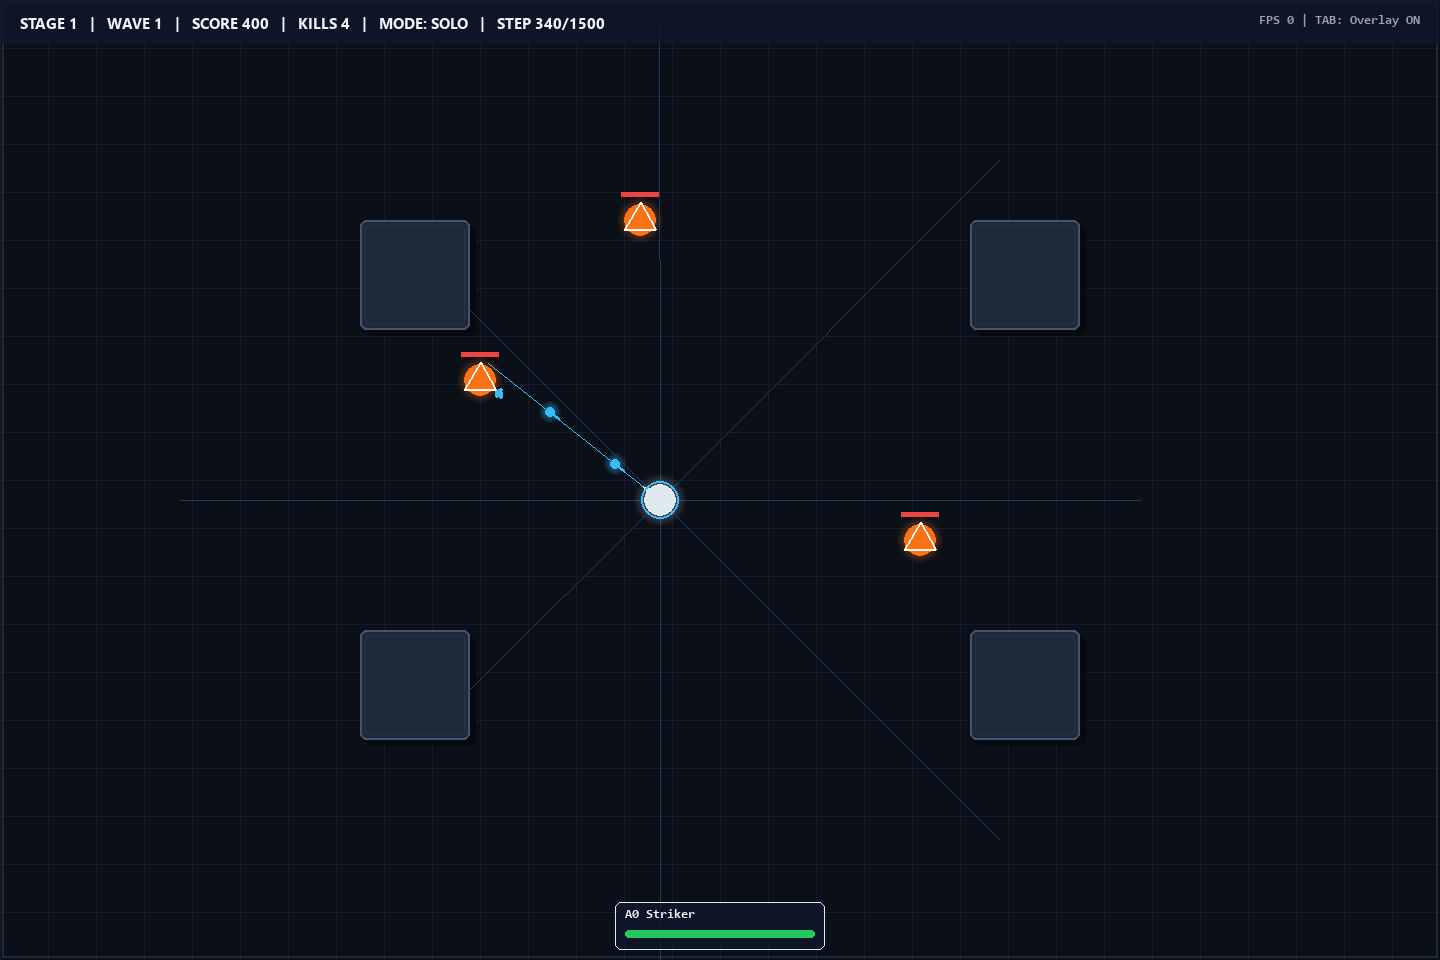
\includegraphics[width=\textwidth]{../assets/screenshots/stage1_cover_combat.png}
\end{minipage}
\hfill
\begin{minipage}[b]{0.48\textwidth}
    \centering
    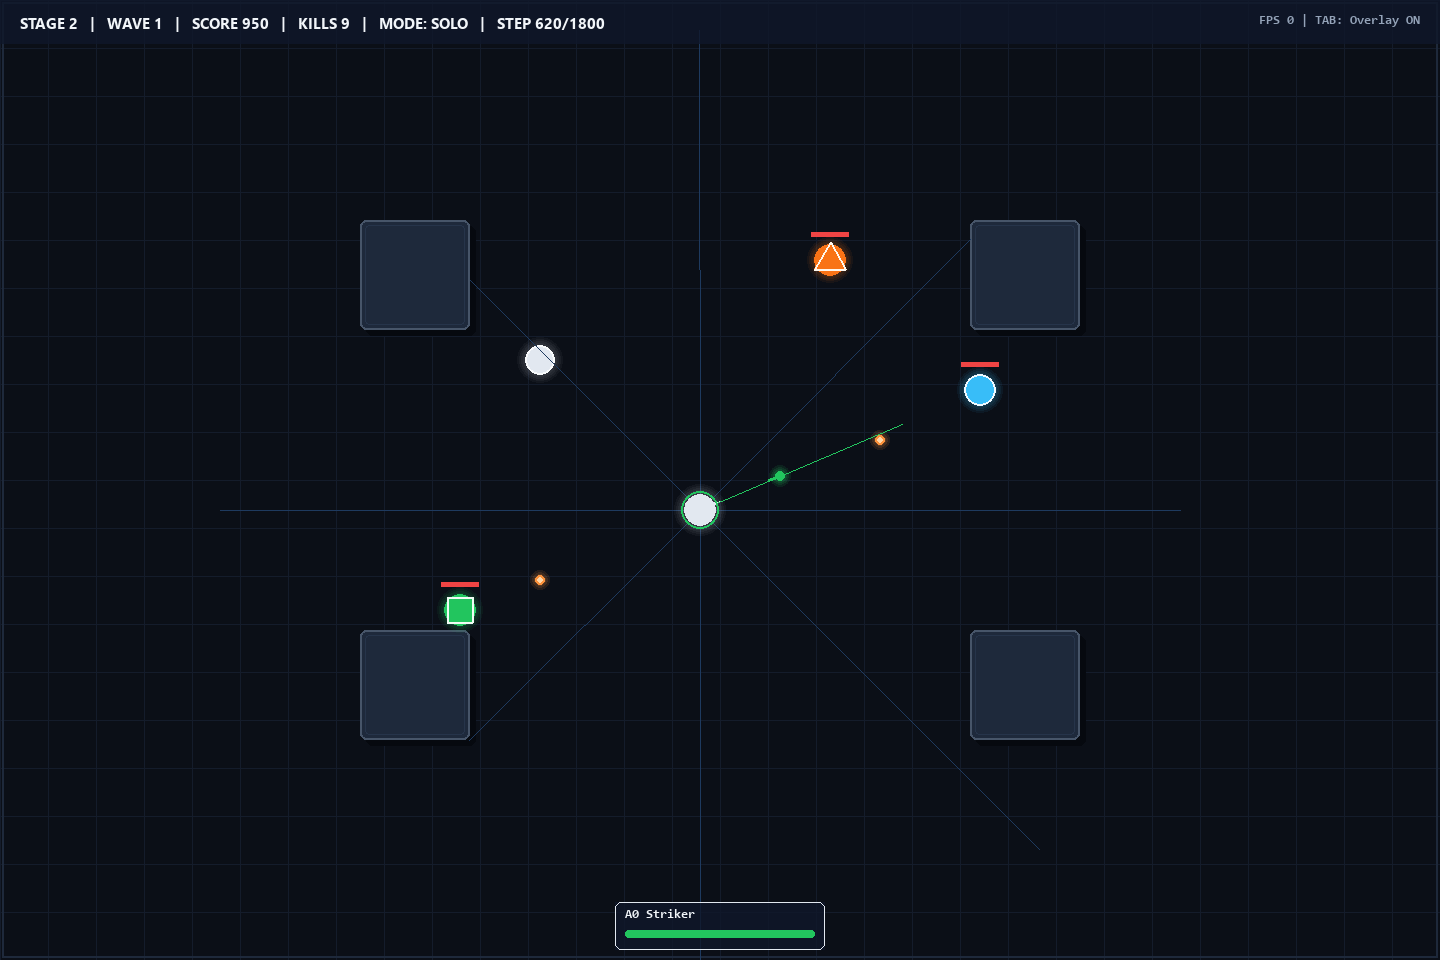
\includegraphics[width=\textwidth]{../assets/screenshots/stage2_elemental_mastery.png}
\end{minipage}
\caption{In-game captures of single-agent curriculum stages with the 8-ray LIDAR and aim-laser overlay active. \textbf{Left (Stage 1):} \texttt{A0 Striker} engages three \texttt{Fire} enemies around four cover pillars using \texttt{Water} projectiles. \textbf{Right (Stage 2):} \texttt{A0 Striker} tracks mixed \texttt{Fire}, \texttt{Water}, and \texttt{Grass} enemies while dodging incoming shots and avoiding a neutral white ally.}
\label{fig:screenshots-single}
\end{figure}

\begin{figure}[t]
\centering
\begin{minipage}[b]{0.48\textwidth}
    \centering
    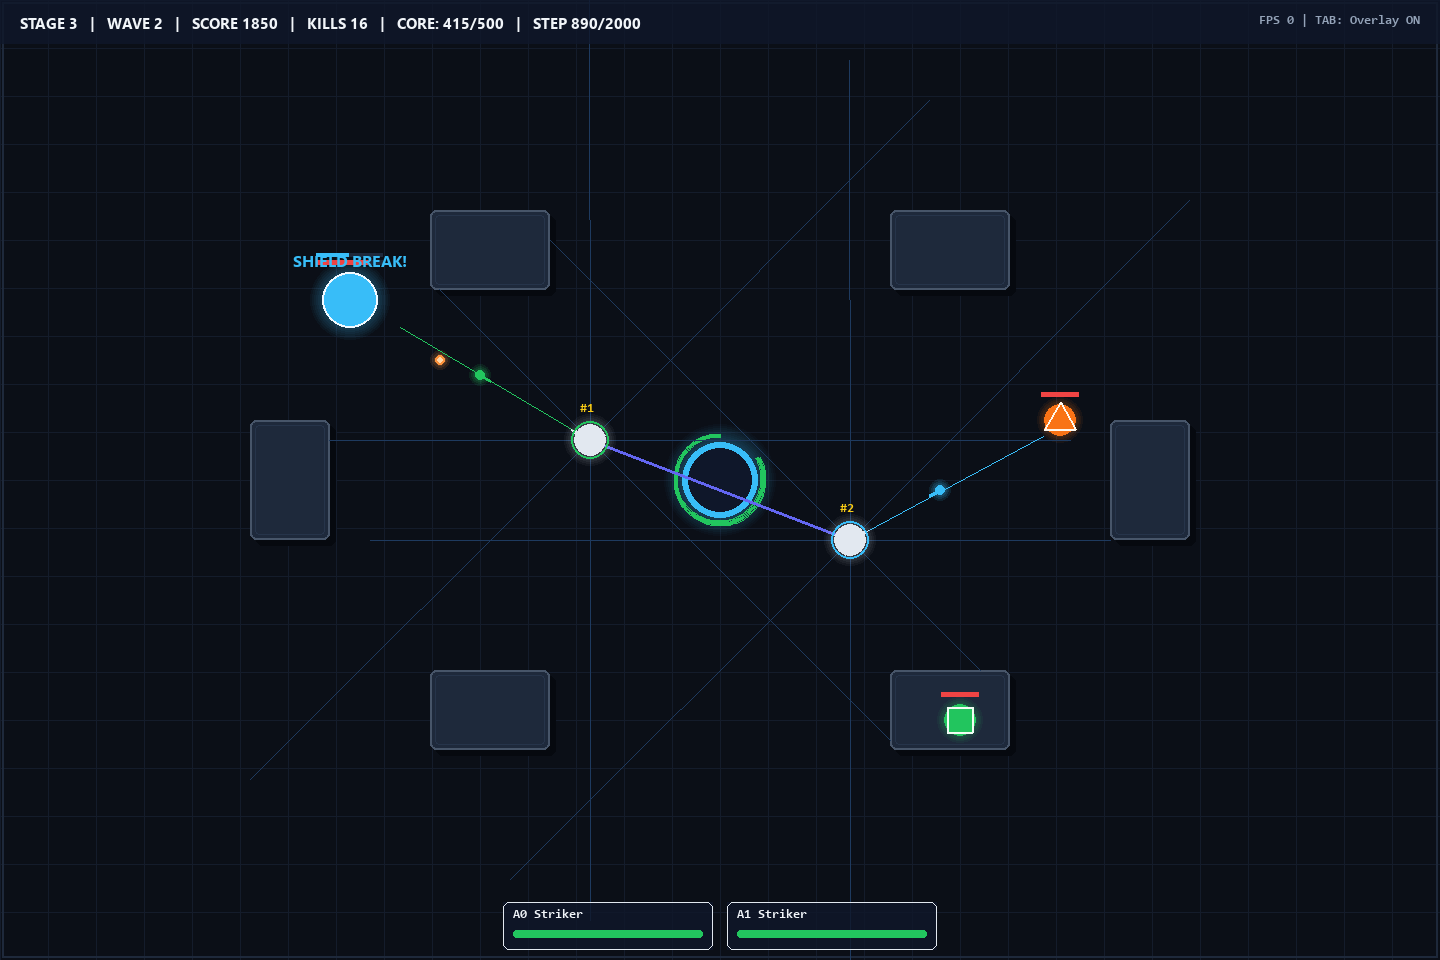
\includegraphics[width=\textwidth]{../assets/screenshots/stage3_coop_boss_overlay.png}
\end{minipage}
\hfill
\begin{minipage}[b]{0.48\textwidth}
    \centering
    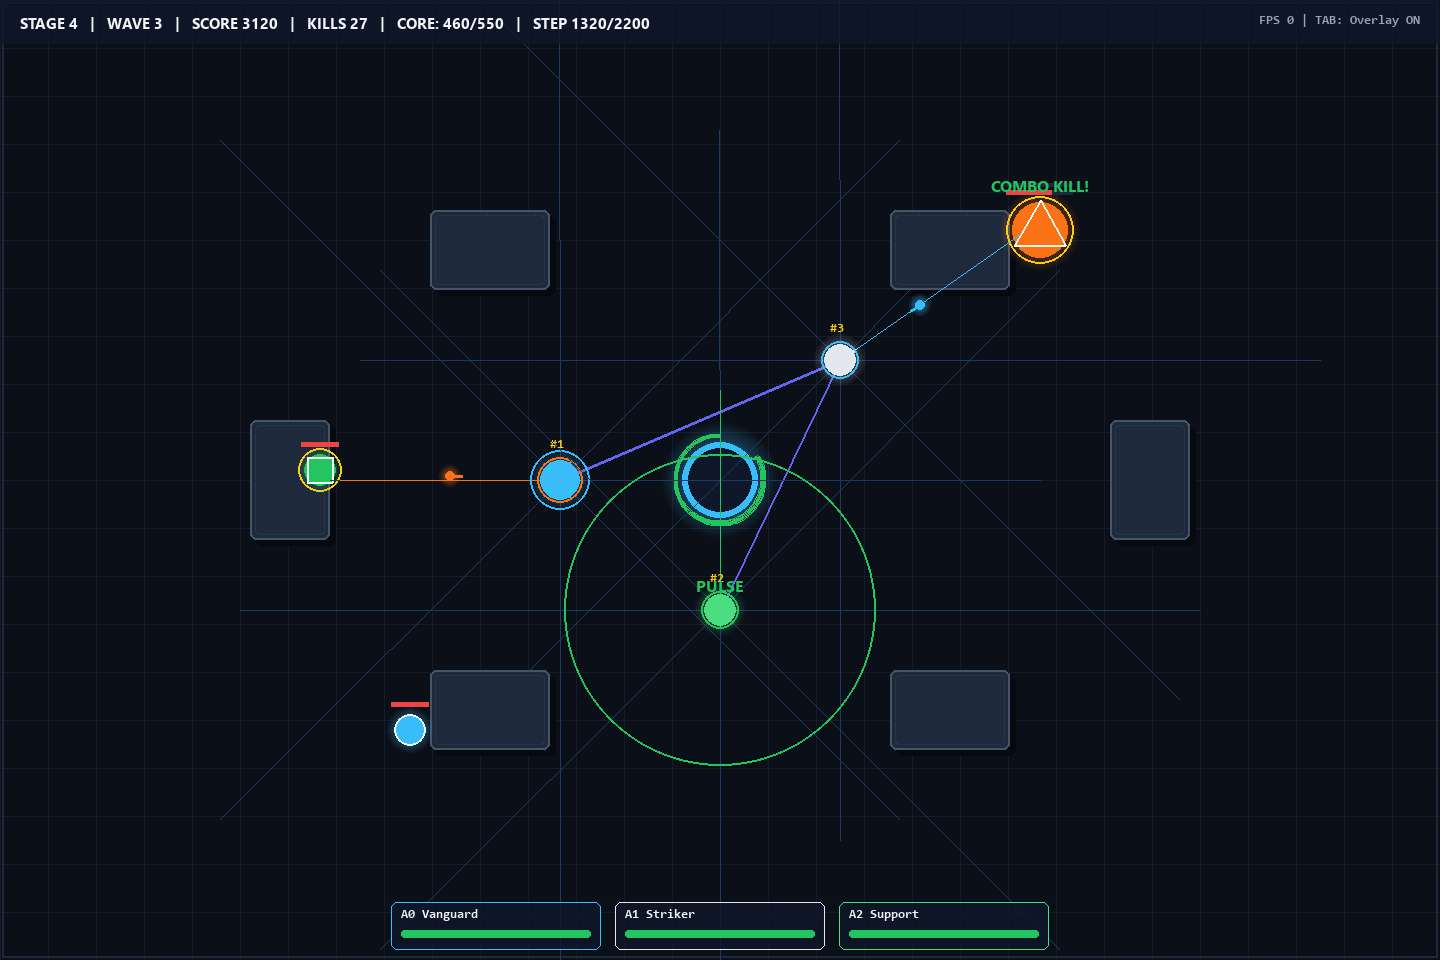
\includegraphics[width=\textwidth]{../assets/screenshots/stage4_heterogeneous_squad.png}
\end{minipage}
\caption{In-game captures of cooperative multi-agent stages with the MARL explainability overlay enabled. \textbf{Left (Stage 3):} Two \texttt{Striker} agents (\texttt{\#1}, \texttt{\#2}) defend the Central Core (\texttt{415/500} HP) across six cover blocks as \texttt{\#1} triggers a \texttt{SHIELD BREAK!} on a \texttt{Water} boss with \texttt{Grass} bolts. \textbf{Right (Stage 4):} \texttt{A0 Vanguard} (\texttt{\#1}, Aegis Shield active), \texttt{A2 Support} (\texttt{\#2}, emitting a green Repair and Mark \texttt{PULSE}), and \texttt{A1 Striker} (\texttt{\#3}) score a \texttt{COMBO KILL!} on a marked \texttt{Fire} boss.}
\label{fig:screenshots-coop}
\end{figure}

\subsection{Formal Dec-POMDP Components}

\paragraph{Elemental Graph and Boss Shields.}
Weapons and enemies belong to $\{0: \text{Water}, 1: \text{Grass}, 2: \text{Fire}\}$, governed by cyclic advantage: \textbf{Water} beats \textbf{Fire}, \textbf{Grass} beats \textbf{Water}, and \textbf{Fire} beats \textbf{Grass}. Wrong-element hits deal zero hull damage and incur an \texttt{IMMUNE} penalty. In Stages 3 and 4, periodic shielded bosses spawn with an elemental shield ($\ge 110$ HP) that absorbs $90\%$ of hull damage until shattered by the counter-element, opening a $160$-tick vulnerability window ($+35\%$ team damage; $+35\%$ additional bonus for \texttt{Striker}) and awarding team shield-break and combo-kill bonuses.

\paragraph{Factored Action Space.}
Each agent $i$ outputs a 4-tuple from \texttt{MultiDiscrete([3, 3, 32, 4])}: horizontal move $a_{i,0} \in \{-1, 0, +1\}$, vertical move $a_{i,1} \in \{-1, 0, +1\}$ (diagonal vectors normalized to unit speed), aim bin $a_{i,2} \in \{0, \dots, 31\}$ mapping to $\theta_k = 2\pi k / 32$ ($11.25^\circ$ resolution), and fire/ability command $a_{i,3} \in \{0, 1, 2, 3\}$, where $0$ holds fire (and triggers the Stage 4 class tactical ability when off cooldown with threats or wounded allies nearby) and $1, 2, 3$ fire Water, Grass, or Fire.

\paragraph{Local Observation vs. Privileged Global State.}
To enable direct policy transfer from Stage 2 to Stages 3 and 4 without reshaping tensors, every agent receives a fixed $129$-dimensional \texttt{float32} vector $o_i^t \in [-1, 1]^{129}$:
\begin{itemize}
    \item \textbf{Self-State (14):} normalized $(x, y)$, velocity $(v_x, v_y)$, HP ratio, fire and ability cooldowns, alive flag, last fired weapon one-hot (3), and class role one-hot (3).
    \item \textbf{Central Core State (5):} relative $(\Delta x, \Delta y)$, normalized distance, Core HP ratio, and under-attack flag (zeroed in Stages 1--2).
    \item \textbf{Obstacle LIDAR (8):} 8-direction raycast distances up to $480\text{ px}$ mapped to $[-1, 1]$.
    \item \textbf{Top-5 Visible Hostiles ($5 \times 15 = 75$):} relative $(\Delta x, \Delta y)$, $(\sin\theta, \cos\theta)$, normalized distance, enemy velocity $(v_x, v_y)$ for target leading, HP ratio, shield ratio, element one-hot (3), boss flag, marked flag, and active/LOS flag. In Stages 3--4 (\texttt{partial\_obs=True}), enemies beyond $760\text{ px}$ or occluded by cover blocks are masked to zero.
    \item \textbf{Teammates / Neutral Allies ($3 \times 9 = 27$):} relative $(\Delta x, \Delta y)$, distance, HP ratio, role/neutral one-hot (4), and alive flag.
\end{itemize}
For centralized training, \texttt{env.state()} exposes the unoccluded global state $s^t$, concatenating all agent states ($N \times 14$), Core state ($5$), all active enemies up to $E_{\max}$ regardless of LOS occlusion ($E_{\max} \times 15$), and global wave progress ($4$).

\paragraph{Decomposed Reward Function.}
Per-step rewards combine individual shaping with shared team outcomes via mixing coefficient $\alpha \in [0, 1]$:
\begin{equation}
r_i^t = (1 - \alpha) r_{i,\text{indiv}}^t + \alpha r_{\text{team}}^t,
\end{equation}
where $r_{i,\text{indiv}}^t$ rewards counter-element hits, target-leading precision, solo kills, Vanguard mitigation, Support repair/mark utility, and trigger discipline while penalizing wrong-element shots, missed shots (scaling softly with cumulative misses), friendly fire, damage taken, and death; $r_{\text{team}}^t$ rewards team eliminations, boss kills, shield breaks, multi-agent combo kills, wave clears, and Core healing while penalizing Core damage, Core loss, and teammate deaths.

\subsection{Stage 4 Heterogeneous Squad Specification}

Table~\ref{tab:stage4-classes} defines the three Stage 4 classes engineered specifically for Milestone 2 heterogeneity studies contrasting parameter-sharing \texttt{MAPPO} against unshared \texttt{HAPPO}/\texttt{HATRPO} and role-conditioned \texttt{RoMAT}/\texttt{PMAT}.

\begin{table}[t]
\centering
\caption{Stage 4 heterogeneous squad attributes and tactical abilities triggered via $a_{i,3} = 0$.}
\label{tab:stage4-classes}
\small
\begin{tabular}{@{}lcccl@{}}
\toprule
Class & Max HP & Speed & Fire / Abil. CD & Tactical Ability ($a_{i,3} = 0$) \\
\midrule
Vanguard & 180 & 3.5 & 16 / 140 & Aegis Shield: 90 ticks, 65\% damage mitigation, pulls aggro within $420\text{ px}$ \\
Striker & 100 & 4.8 & 12 / 90 & High-mobility DPS ($+35\%$ bonus damage vs. shattered boss shields) \\
Support & 115 & 4.3 & 14 / 120 & Repair \& Mark Pulse ($+26$ Core HP, $+22$ ally HP, marks 2 enemies $+35\%$ dmg) \\
\bottomrule
\end{tabular}
\end{table}

\section{Milestone 1 Experimental Setup and Statistical Protocol}

All Milestone 1 runs executed on a Windows workstation equipped with an NVIDIA GeForce RTX 3060 GPU (12 GB VRAM), Python 3.11.18, and PyTorch 2.6.0+cu124. Every experiment is specified by a versioned YAML configuration and deterministic seeding across Python \texttt{random}, NumPy, PyTorch, and vectorized environment workers.

Following Agarwal et al.~\cite{agarwal2021rliable} and Gorsane et al.~\cite{gorsane2022marleval}, we evaluate checkpoints across multiple fixed seeds and report Interquartile Mean (IQM) with $95\%$ stratified bootstrap confidence intervals ($B = 2{,}000$ resamples), alongside mean win rate, Core survival ratio, elemental accuracy, kills per episode, and simulation throughput (FPS). Milestone 1 deliberately uses compact training budgets—$60{,}000$ steps in Stage 1, $80{,}000$ steps in Stage 2 (3 seeds each: \texttt{[0, 1, 2]}), and $40{,}000$--$40{,}960$ steps in Stage 3 (2 seeds: \texttt{[0, 1]})—to verify environment dynamics, reward scaling, and early algorithm differentiation before launching $500{,}000+$ step Milestone 2 sweeps.

\section{Quantitative Results and Qualitative Analysis}

\subsection{Single-Agent Benchmarks (Stages 1 and 2)}

Table~\ref{tab:stage12-results} reports Milestone 1 results for Stages 1 and 2, paired with training curves in Figures~\ref{fig:stage1-curves} and~\ref{fig:stage2-curves}. Single-agent CPU \texttt{SubprocVecEnv} rollouts ran at $1{,}878$--$2{,}979$ FPS in Stage 1 and $2{,}093$--$2{,}776$ FPS in Stage 2.

\begin{table}[t]
\centering
\caption{Milestone 1 single-agent results on Stage 1 (60,000 steps, 3 seeds) and Stage 2 (80,000 steps, 3 seeds). Values show IQM with 95\% bootstrap CIs and evaluation means.}
\label{tab:stage12-results}
\small
\begin{tabular}{@{}llccccc@{}}
\toprule
Stage & Agent & Final Return IQM [95\% CI] & Best Return IQM [95\% CI] & Win Rate & Elem. Acc. & Kills/Ep \\
\midrule
Stage 1 & HEURISTIC & $21.63\;[20.19, 22.57]$ & --- & $97.9\%$ & $100.0\%$ & $21.1$ \\
Stage 1 & PPO (60k) & $-4.47\;[-4.95, -4.00]$ & $-3.46\;[-4.00, -3.15]$ & $0.0\%$ & $34.7\%$ & $0.1$ \\
Stage 1 & RANDOM & $-3.04\;[-3.08, -2.99]$ & --- & $0.0\%$ & $32.6\%$ & $0.0$ \\
\midrule
Stage 2 & HEURISTIC & $9.70\;[9.19, 10.58]$ & --- & $0.0\%$ & $99.7\%$ & $10.9$ \\
Stage 2 & PPO (80k) & $-3.48\;[-3.89, -3.25]$ & $-2.98\;[-3.30, -2.73]$ & $0.0\%$ & $17.8\%$ & $0.0$ \\
Stage 2 & RANDOM & $-2.72\;[-2.83, -2.64]$ & --- & $0.0\%$ & $31.6\%$ & $0.0$ \\
\bottomrule
\end{tabular}
\end{table}

\begin{figure}[t]
\centering
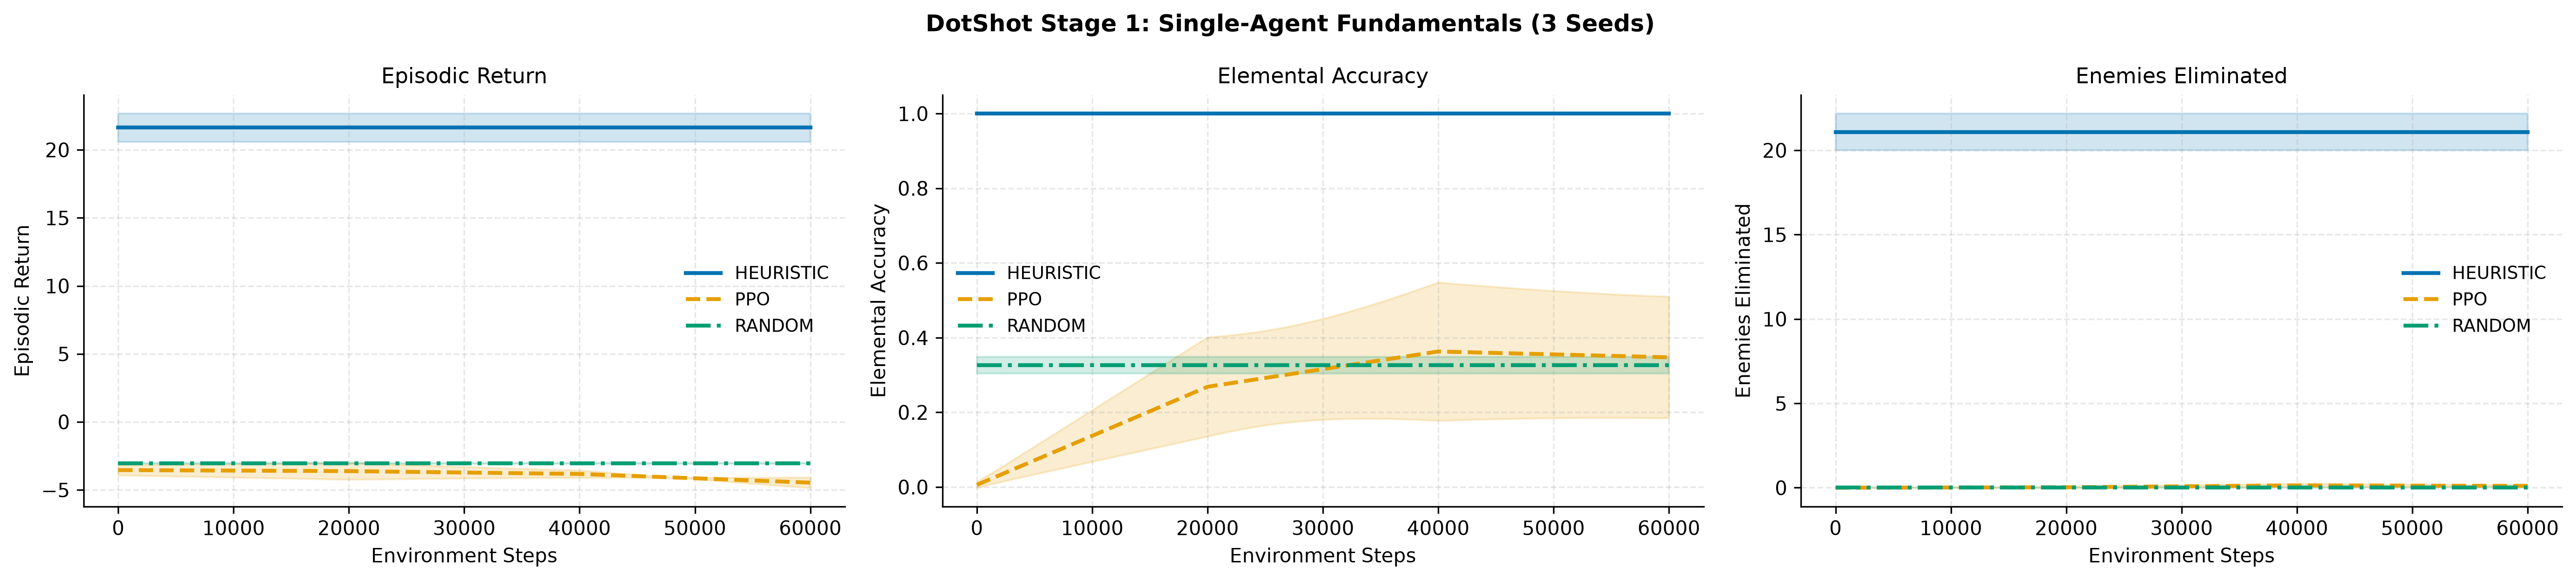
\includegraphics[width=\textwidth]{../assets/figures/stage1_learning_curves.png}
\caption{Stage 1 single-agent learning curves across 3 seeds (0--60,000 environment steps). While the scripted \texttt{HEURISTIC} maintains $21.63$ return, $100.0\%$ elemental accuracy, and $21.1$ kills/episode, \texttt{PPO} raises elemental accuracy toward $34.7\%$ at $40{,}000$--$60{,}000$ steps while its return stays below \texttt{RANDOM} due to early miss penalties across 32 aim bins.}
\label{fig:stage1-curves}
\end{figure}

\begin{figure}[t]
\centering
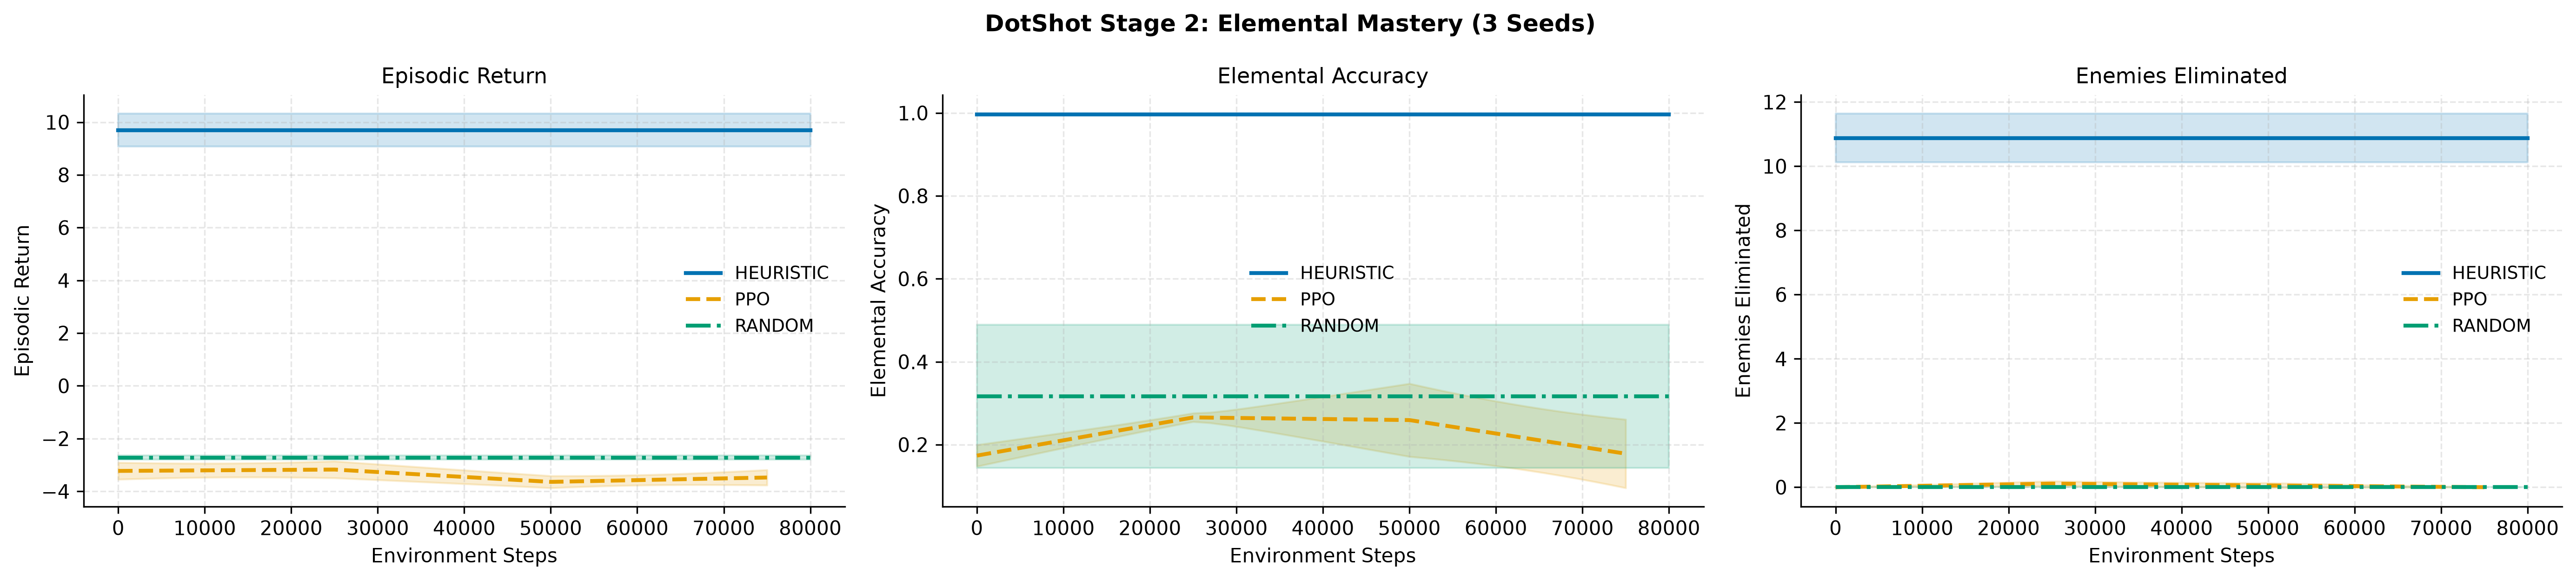
\includegraphics[width=\textwidth]{../assets/figures/stage2_learning_curves.png}
\caption{Stage 2 single-agent learning curves across 3 seeds (0--80,000 environment steps). Adding multi-element spawns, enemy projectiles, and neutral allies lowers \texttt{HEURISTIC} win rate to $0.0\%$ ($9.70$ return, $10.9$ kills/episode), while early \texttt{PPO} remains at $-3.48$ return and $17.8\%$ elemental accuracy over the short 80k horizon.}
\label{fig:stage2-curves}
\end{figure}

Three behavioral patterns emerge from Figures~\ref{fig:stage1-curves} and~\ref{fig:stage2-curves}:
\begin{itemize}
    \item \textbf{Factored Exploration Bottleneck vs. Miss Penalties:} In Stage 1, \texttt{PPO} at $60{,}000$ steps achieves lower return ($-4.47$) than a uniform \texttt{RANDOM} baseline ($-3.04$), even though \texttt{PPO} scores $0.1$ kills/episode and lifts elemental accuracy to $34.7\%$. Under a 42-logit factored policy spanning 32 aim bins ($11.25^\circ$ width) and 4 weapon choices, an untrained policy fires roughly $75\%$ of ticks while aiming inaccurately. DotShot's per-shot miss penalty accumulates steadily whenever shots miss narrow enemy hitboxes, penalizing an active early policy more heavily than \texttt{RANDOM} movement that happens to wander away from triggers or die sooner.
    \item \textbf{Stage 2 Difficulty Calibration:} Even the rule-based \texttt{HEURISTIC} drops from a $97.9\%$ win rate and $21.1$ kills/episode in Stage 1 to a $0.0\%$ win rate, $9.70$ return, and $10.9$ kills/episode in Stage 2, despite $99.7\%$ elemental accuracy. Incoming enemy projectiles combined with neutral allies and six simultaneous multi-element foes require genuine projectile dodging and positioning rather than naive nearest-enemy kiting.
    \item \textbf{Horizon Requirements for 32-Bin Aiming:} With $1{,}152$ implicit action combinations and sparse projectile hits early in training, $60{,}000$--$80{,}000$ environment steps constitute fewer than $100$ policy updates—insufficient for \texttt{PPO} to lock onto leading angles before the miss penalty shapes trigger restraint.
\end{itemize}

\subsection{Cooperative Stage 3 Smoke Benchmark}

Table~\ref{tab:stage3-smoke} presents the Stage 3 cooperative defense smoke benchmark across five algorithms trained for $40{,}000$--$40{,}960$ steps on the RTX 3060 GPU across 2 seeds (\texttt{[0, 1]}), and Figure~\ref{fig:stage3-curves} plots their learning trajectories.

\begin{table}[t]
\centering
\caption{Milestone 1 Stage 3 cooperative smoke benchmark (40,000--40,960 env steps on RTX 3060 CUDA, 2 seeds). Values report IQM [95\% bootstrap CI], Core HP survival ratio, elemental accuracy, kills/episode, and training throughput.}
\label{tab:stage3-smoke}
\small
\begin{tabular}{@{}lcccccc@{}}
\toprule
Algorithm & Final Return IQM [95\% CI] & Best Return IQM [95\% CI] & Core HP & Elem. Acc. & Kills/Ep & Throughput \\
\midrule
MAT & $-2.16\;[-2.26, -2.06]$ & $-2.06\;[-2.26, -1.86]$ & $21.2\%$ & $31.7\%$ & $0.1$ & 201--337 FPS \\
QMIX (Branching) & $-2.19\;[-2.33, -2.04]$ & $-2.02\;[-2.04, -1.99]$ & $22.7\%$ & $52.1\%$ & $0.1$ & 397--470 FPS \\
MAPPO & $-2.30\;[-2.40, -2.21]$ & $-2.20\;[-2.21, -2.20]$ & $29.3\%$ & $32.2\%$ & $0.1$ & 509--713 FPS \\
IPPO & $-2.52\;[-2.53, -2.50]$ & $-2.36\;[-2.53, -2.20]$ & $7.0\%$ & $30.1\%$ & $0.1$ & 533--836 FPS \\
HAPPO & $-2.78\;[-3.12, -2.44]$ & $-2.20\;[-2.29, -2.12]$ & $2.2\%$ & $16.8\%$ & $0.1$ & 331--525 FPS \\
\bottomrule
\end{tabular}
\end{table}

\begin{figure}[t]
\centering
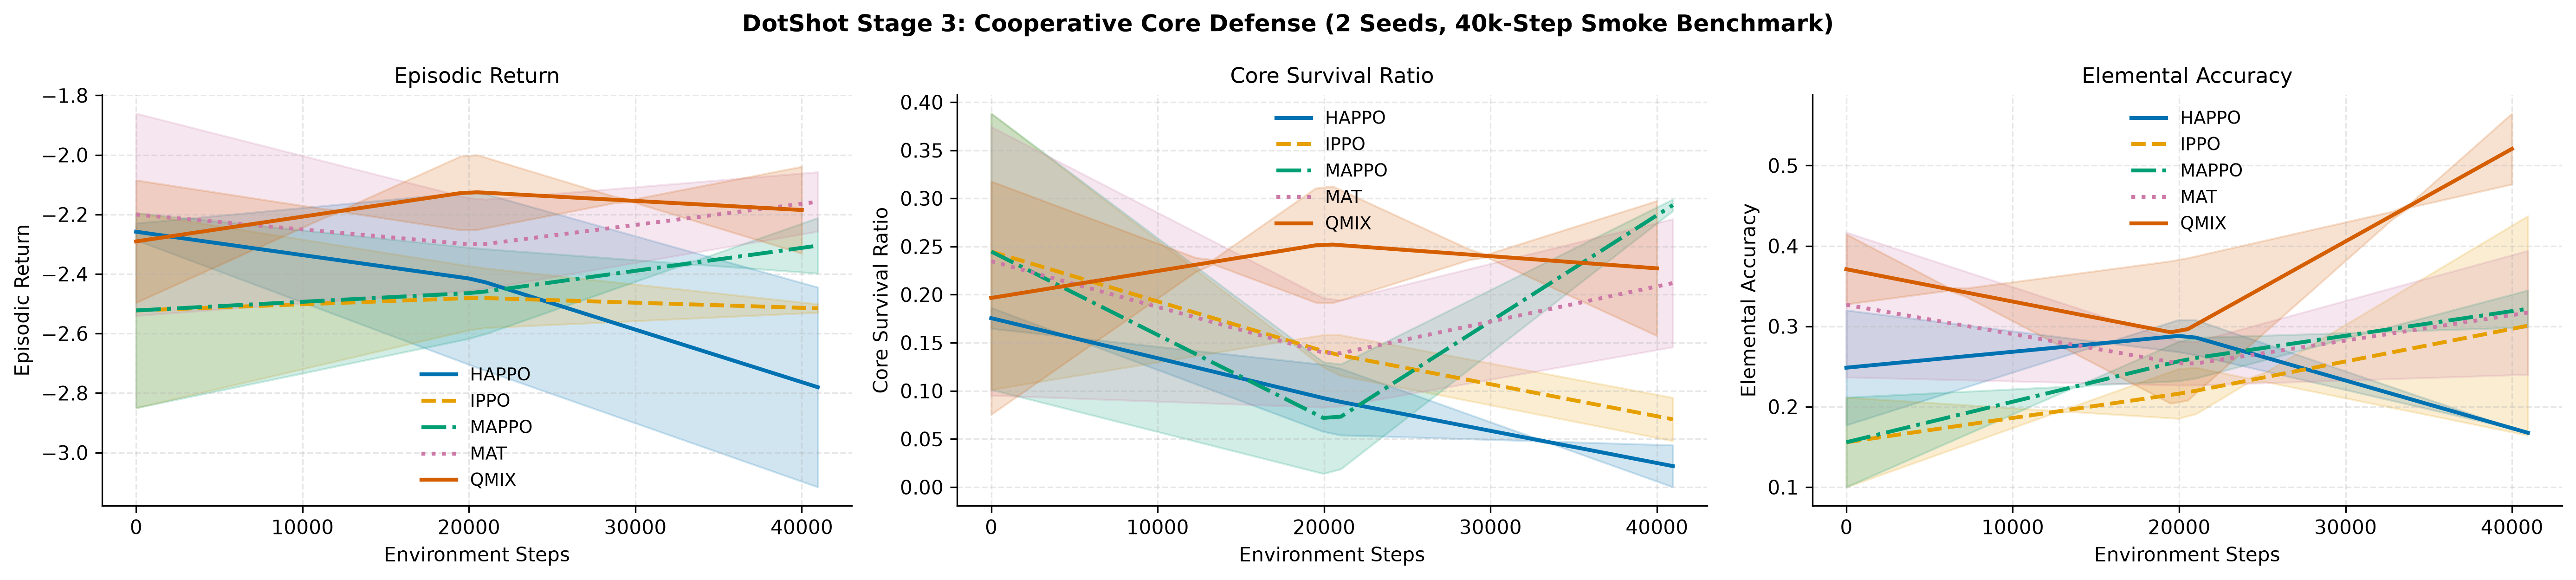
\includegraphics[width=\textwidth]{../assets/figures/stage3_marl_smoke_comparison.png}
\caption{Stage 3 cooperative smoke comparison across 2 seeds (0--40,960 environment steps). \texttt{MAT} ($-2.16$) and \texttt{Branching-QMIX} ($-2.19$) lead in episodic return, \texttt{MAPPO} climbs steadily to $29.3\%$ Core HP retention, and \texttt{Branching-QMIX} reaches $52.1\%$ elemental accuracy, whereas \texttt{IPPO} ($7.0\%$ Core HP) and unshared \texttt{HAPPO} ($2.2\%$ Core HP) lose Core protection within the 40k smoke budget.}
\label{fig:stage3-curves}
\end{figure}

Even within a $40{,}000$-step smoke horizon where win rates remain $0.0\%$ and kills average $0.1$ per episode, four clear qualitative distinctions appear across the five MARL families:

\begin{enumerate}
    \item \textbf{CTDE Critics Preserve the Central Core Better Than IPPO:} Every shared-parameter or sequence-modeled CTDE method—\texttt{MAPPO} ($29.3\%$ Core HP), \texttt{Branching-QMIX} ($22.7\%$), and \texttt{MAT} ($21.2\%$)—retains more than triple the Core health of decentralized \texttt{IPPO} ($7.0\%$) at $40{,}960$ steps. Conditioning on the privileged global state $s^t$ lets centralized critics and hypernetworks penalize Core damage consistently even when enemies approach from outside an individual Striker's line-of-sight mask.
    \item \textbf{Off-Policy Branching-QMIX Accelerates Weapon Selection:} \texttt{Branching-QMIX} reaches $52.1\%$ elemental accuracy by $40{,}000$ steps, outperforming all on-policy methods by roughly $20$ percentage points ($30.1\%$--$32.2\%$). Because a Branching Dueling Q-head separates the 4-way weapon choice from the 32-bin aim head and reuses off-policy transitions in replay, it identifies counter-element payoffs faster than on-policy rollouts.
    \item \textbf{MAT and MAPPO Show Complementary Early Strengths:} \texttt{MAT} records the highest final IQM return ($-2.16$, CI $[-2.26, -2.06]$) at the cost of lower simulation throughput ($201$--$337$ FPS) due to Transformer encoder-decoder passes. \texttt{MAPPO} runs nearly twice as fast ($509$--$713$ FPS) and displays the steepest positive slope on both episodic return (rising from $-2.53$ to $-2.30$) and Core survival ($29.3\%$) between $20{,}000$ and $40{,}960$ steps.
    \item \textbf{Why Unshared HAPPO Lags at 40k Steps:} \texttt{HAPPO} finishes lowest in return ($-2.78$), Core HP ($2.2\%$), and elemental accuracy ($16.8\%$). Unlike \texttt{MAPPO} and \texttt{MAT}, \texttt{HAPPO} trains separate actor networks $\theta^0$ and $\theta^1$ without parameter sharing. In homogeneous Stage 3, disabling parameter sharing halves the effective gradient data per actor network and compounds variance through the sequential importance-sampling multiplier $M^{i_{1:m}}$, slowing early adaptation over a $40{,}000$-step smoke run.
\end{enumerate}

\subsection{Design Predictions for Milestone 2 (500k+ Steps and Stage 4)}

These Milestone 1 diagnostics yield two testable hypotheses for Milestone 2 full-horizon runs ($500{,}000+$ environment steps across 5 seeds):
\begin{itemize}
    \item \textbf{Stage 3 Convergence:} Once Stage 1--2 Striker aiming warms up past the initial miss-penalty trough, shared-weight \texttt{MAPPO}, \texttt{Branching-QMIX}, and \texttt{MAT} should separate on boss shield-break timing and combo kills, while \texttt{HAPPO} should close its early sample-efficiency gap against \texttt{MAPPO}.
    \item \textbf{Stage 4 Heterogeneity Inversion:} When \texttt{Vanguard}, \texttt{Striker}, and \texttt{Support} introduce asymmetric speeds, hitboxes, and $a_{i,3} = 0$ abilities (Table~\ref{tab:stage4-classes}), parameter sharing in \texttt{MAPPO} will experience gradient interference between frontline aggro-tanking and rear-line pulse healing, creating the exact regime where unshared \texttt{HAPPO}/\texttt{HATRPO}~\cite{kuba2022happo,zhong2024harl} and role-conditioned \texttt{RoMAT}/\texttt{PMAT} should overtake homogeneous baselines.
\end{itemize}

\section{Limitations and Future Work}

Milestone 1 intentionally prioritizes structural validation over asymptotic convergence. First, $40{,}000$--$80{,}000$ environment steps are too short to learn 32-bin target leading from scratch alongside elemental switching, leaving RL win rates at $0.0\%$ in this preliminary pass. Second, Stage 3 ran on 2 seeds per algorithm; widening to 5+ seeds in Milestone 2 will tighten bootstrap confidence intervals. Third, Stage 4 heterogeneous squad benchmarks and curriculum transfer from Stage 2 Striker checkpoints remain to be executed in Milestone 2, alongside distilling centralized \texttt{MAT}/\texttt{PMAT} policies into fully decentralized actors for bandwidth-constrained deployment.

\bibliographystyle{plainnat}
\bibliography{../references}

\end{document}
